\documentclass[10pt,a4paper]{article}
\usepackage[margin=2cm]{geometry}
\usepackage[T1]{fontenc}
\usepackage{lmodern}
\usepackage{amsmath,amssymb}
\usepackage{booktabs,tabularx,array}
\usepackage{graphicx}
\usepackage{xcolor}
\usepackage[round]{natbib}
\usepackage{tikz}
\usetikzlibrary{arrows.meta,positioning,calc}
\usepackage{caption}
\usepackage[colorlinks=true,allcolors=blue!50!black]{hyperref}
\usepackage{url}
\graphicspath{{../stats/figs/}}
\captionsetup{font=small,labelfont=bf,skip=3pt}
\setlength{\textfloatsep}{8pt plus 2pt minus 2pt}\setlength{\floatsep}{6pt}\setlength{\intextsep}{6pt}

% ---- figures / tables produced by the scripts; the article compiles even before they exist
\newcommand{\maybefig}[3]{% file, width, caption-label
  \IfFileExists{../stats/figs/#1}{\includegraphics[width=#2\textwidth]{#1}}%
  {\fbox{\parbox{0.8\textwidth}{\centering\small [figure \texttt{\detokenize{#1}} not generated yet -- run \texttt{analyze.py}]}}}}
\newcommand{\maybetab}[1]{%
  \IfFileExists{../stats/tabs/#1}{\input{../stats/tabs/#1}}%
  {\fbox{\parbox{0.8\textwidth}{\centering\small [table \texttt{\detokenize{#1}} not generated yet -- run \texttt{analyze.py}]}}}}

\newcommand{\E}{\mathbb{E}}
\newcommand{\R}{\mathbb{R}}
\newcommand{\dd}{\,\mathrm{d}}
\newcommand{\Tb}{\bar T}

\title{\textbf{A Fractional Delayed Impulsive Model of Interacting Earthquake Faults:\\ Probabilistic Forecasting and Statistical Validation}}
\author{Mohamad Yamen Al-Mohamad\\
\small Department of Statistics, University of Tabriz, Tabriz, Iran\\
\small \texttt{yamenmohamad@tabrizu.ac.ir}}
\date{\today}

%%% ---------- Figure A: the problem ----------
\newcommand{\figProblem}{%
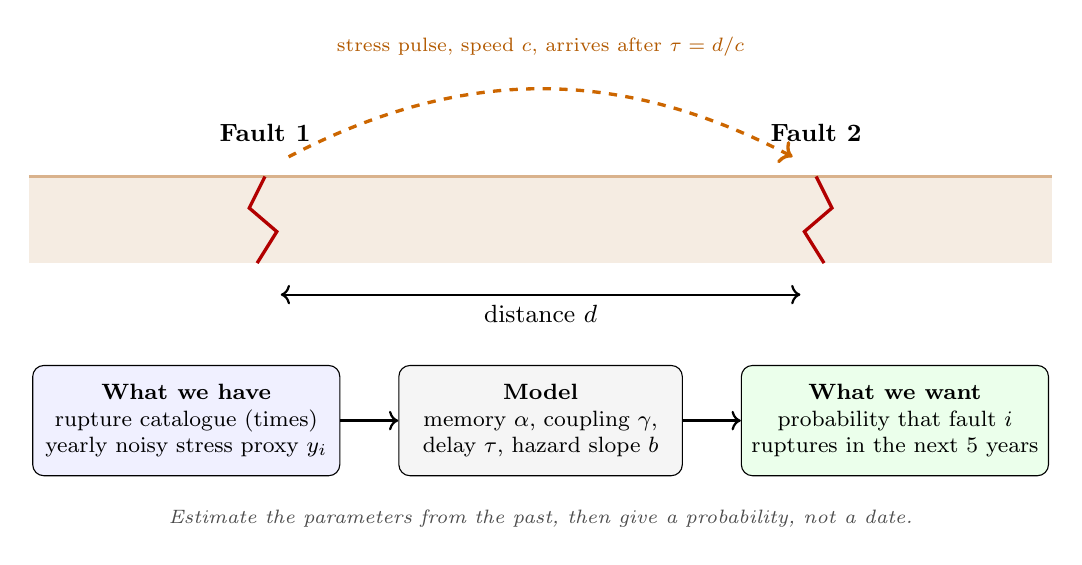
\begin{tikzpicture}[x=1cm,y=1cm,
  lab/.style={font=\small,align=center},
  bx/.style={font=\footnotesize,align=center,draw,rounded corners,minimum height=1.4cm},
  note/.style={font=\scriptsize,align=center,text=black!70}]
  % ground
  \fill[brown!15] (0,0) rectangle (13,-1.1);
  \draw[brown!60,thick] (0,0)--(13,0);
  % fault 1 and 2 (zig-zag lines going down)
  \draw[red!70!black,very thick] (3,0)--(2.8,-0.4)--(3.15,-0.7)--(2.9,-1.1);
  \draw[red!70!black,very thick] (10,0)--(10.2,-0.4)--(9.85,-0.7)--(10.1,-1.1);
  \node[lab] at (3,0.55) {\textbf{Fault 1}};
  \node[lab] at (10,0.55) {\textbf{Fault 2}};
  % distance
  \draw[<->,thick] (3.2,-1.5)--node[below,lab]{distance $d$}(9.8,-1.5);
  % pulse
  \draw[->,orange!80!black,very thick,dashed] (3.3,0.25) .. controls (5.5,1.4) and (7.5,1.4) .. (9.7,0.25);
  \node[note,orange!70!black] at (6.5,1.65) {stress pulse, speed $c$, arrives after $\tau=d/c$};
  % what we see
  \node[bx,fill=blue!6,minimum width=3.9cm] (obs) at (2.0,-3.1)
     {\textbf{What we have}\\ rupture catalogue (times)\\ yearly noisy stress proxy $y_i$};
  \node[bx,fill=gray!8,minimum width=3.6cm] (mod) at (6.5,-3.1)
     {\textbf{Model}\\ memory $\alpha$, coupling $\gamma$,\\ delay $\tau$, hazard slope $b$};
  \node[bx,fill=green!8,minimum width=3.9cm] (q) at (11.0,-3.1)
     {\textbf{What we want}\\ probability that fault $i$\\ ruptures in the next 5 years};
  \draw[->,thick] (obs)--(mod);
  \draw[->,thick] (mod)--(q);
  \node[note] at (6.5,-4.35) {\emph{Estimate the parameters from the past, then give a probability, not a date.}};
\end{tikzpicture}}

%%% ---------- Figure B: stress cycle, memory, hazard ----------
\newcommand{\figCycle}{%
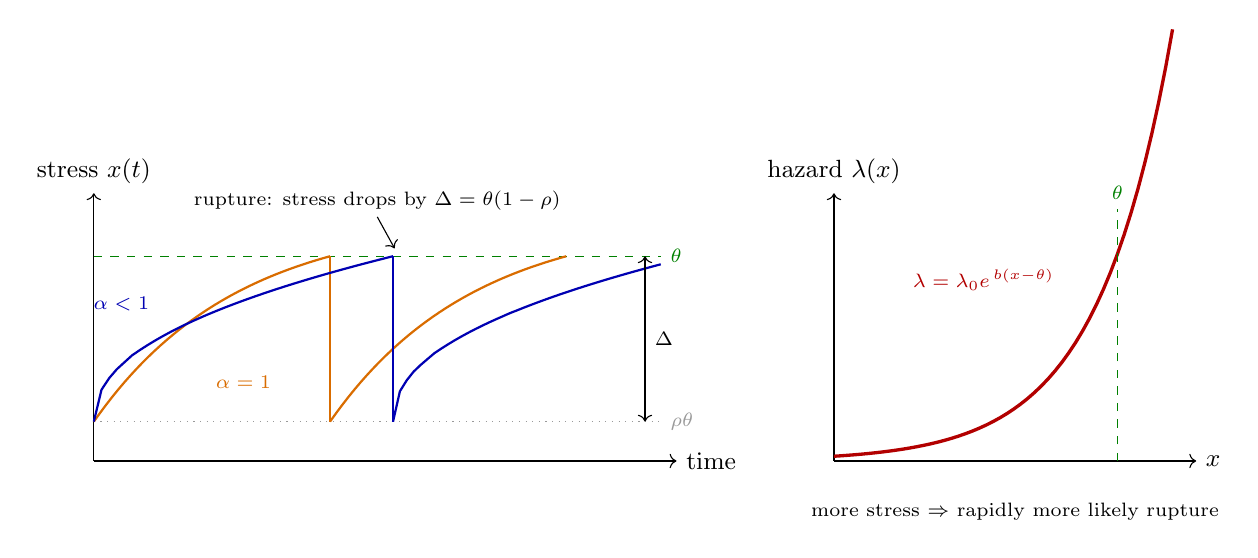
\begin{tikzpicture}[x=1.0cm,y=1.0cm,font=\small]
  % --- left: stress cycles
  \draw[->] (0,0)--(7.4,0) node[right]{time};
  \draw[->] (0,0)--(0,3.4) node[above]{stress $x(t)$};
  \draw[green!50!black,dashed] (0,2.6)--(7.2,2.6) node[right,font=\scriptsize]{$\theta$};
  \draw[black!40,dotted] (0,0.5)--(7.2,0.5) node[right,font=\scriptsize]{$\rho\theta$};
  % no memory (alpha=1): classical saturating curve, two cycles
  \draw[thick,orange!85!black] plot[domain=0:3,samples=40] (\x,{0.5+2.1*(1-exp(-0.55*\x))/(1-exp(-0.55*3))});
  \draw[thick,orange!85!black] (3,2.6)--(3,0.5);
  \draw[thick,orange!85!black] plot[domain=0:3,samples=40] ({3+\x},{0.5+2.1*(1-exp(-0.55*\x))/(1-exp(-0.55*3))});
  % with memory: fast start, slow end (power law)
  \draw[thick,blue!70!black] plot[domain=0:3.8,samples=40] (\x,{0.5+2.1*(\x/3.8)^0.45});
  \draw[thick,blue!70!black] (3.8,2.6)--(3.8,0.5);
  \draw[thick,blue!70!black] plot[domain=0:3.4,samples=40] ({3.8+\x},{0.5+2.1*(\x/3.8)^0.45});
  % drop
  \draw[<->] (7.0,0.5)--node[right,font=\scriptsize]{$\Delta$}(7.0,2.6);
  \node[font=\scriptsize,orange!85!black] at (1.9,1.0) {$\alpha=1$};
  \node[font=\scriptsize,blue!70!black] at (0.35,2.0) {$\alpha<1$};
  \node[font=\scriptsize,align=center] at (3.6,3.3) {rupture: stress drops by $\Delta=\theta(1-\rho)$};
  \draw[->,font=\scriptsize] (3.6,3.1)--(3.82,2.7);
  % --- right: hazard
  \begin{scope}[xshift=9.4cm]
    \draw[->] (0,0)--(4.6,0) node[right]{$x$};
    \draw[->] (0,0)--(0,3.4) node[above]{hazard $\lambda(x)$};
    \draw[very thick,red!70!black] plot[domain=0:4.3,samples=50] (\x,{0.06*exp(1.05*\x)});
    \draw[green!50!black,dashed] (3.6,0)--(3.6,3.2) node[above,font=\scriptsize]{$\theta$};
    \node[font=\scriptsize,red!70!black,align=center] at (1.9,2.3) {$\lambda=\lambda_0e^{\,b(x-\theta)}$};
    \node[font=\scriptsize,align=center] at (2.3,-0.65) {more stress $\Rightarrow$ rapidly more likely rupture};
  \end{scope}
\end{tikzpicture}}

%%% ---------- Figure C: delayed pulse timeline ----------
\newcommand{\figDelay}{%
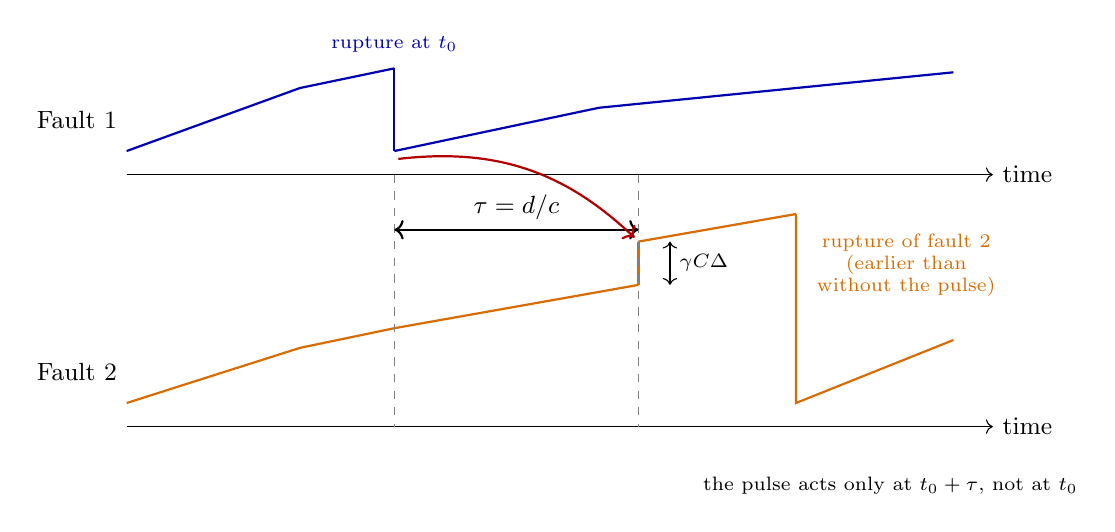
\begin{tikzpicture}[x=1cm,y=1cm,font=\small]
  % fault 1 axis
  \draw[->] (0,3.6)--(11,3.6) node[right]{time};
  \node[left] at (0,4.3) {Fault 1};
  \draw[blue!70!black,thick] (0,3.9)--(2.2,4.7)--(3.4,4.95);
  \draw[blue!70!black,thick] (3.4,4.95)--(3.4,3.9);
  \draw[blue!70!black,thick] (3.4,3.9)--(6,4.45)--(10.5,4.9);
  \node[blue!70!black,font=\scriptsize] at (3.4,5.25) {rupture at $t_0$};
  % fault 2 axis
  \draw[->] (0,0.4)--(11,0.4) node[right]{time};
  \node[left] at (0,1.1) {Fault 2};
  \draw[orange!85!black,thick] (0,0.7)--(2.2,1.4)--(3.4,1.65)--(6.5,2.2);
  \draw[orange!85!black,thick] (6.5,2.2)--(6.5,2.75);       % jump gamma*C*Delta
  \draw[orange!85!black,thick] (6.5,2.75)--(8.5,3.1);
  \draw[orange!85!black,thick] (8.5,3.1)--(8.5,0.7)--(10.5,1.5);
  \node[orange!85!black,font=\scriptsize,align=center] at (9.9,2.45) {rupture of fault 2\\ (earlier than\\ without the pulse)};
  % delay arrows
  \draw[dashed,gray] (3.4,3.6)--(3.4,0.4);
  \draw[dashed,gray] (6.5,3.6)--(6.5,0.4);
  \draw[<->,thick] (3.4,2.9)--node[above]{$\tau=d/c$}(6.5,2.9);
  \draw[->,red!70!black,thick] (3.45,3.8) to[bend left=25] (6.45,2.8);
  \node[red!70!black,font=\scriptsize] at (4.4,3.4) {};
  \draw[<->] (6.9,2.2)--node[right,font=\scriptsize]{$\gamma C\Delta$}(6.9,2.75);
  \node[font=\scriptsize,align=center] at (9.7,-0.35) {the pulse acts only at $t_0+\tau$, not at $t_0$};
\end{tikzpicture}}

%%% ---------- Figure D: inference pipeline ----------
\newcommand{\figPipeline}{%
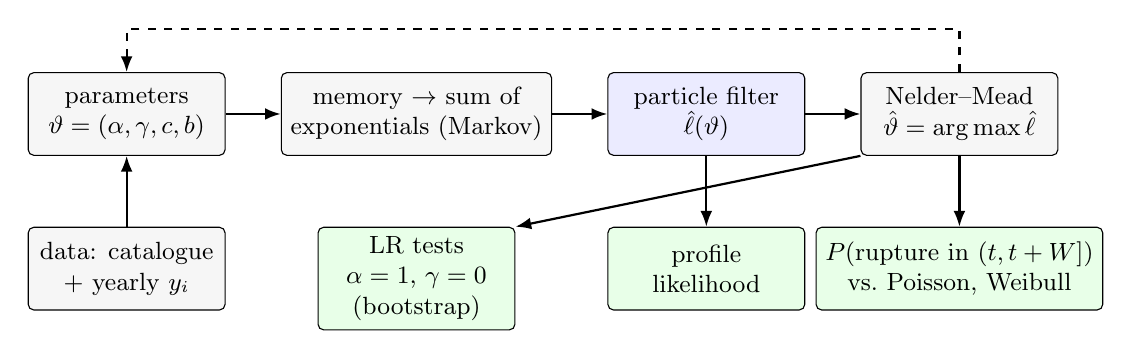
\begin{tikzpicture}[node distance=0.55cm and 0.7cm,
  box/.style={draw,rounded corners=2pt,align=center,minimum height=1.05cm,minimum width=2.5cm,font=\small,fill=gray!7},
  hi/.style={box,fill=blue!8},
  outb/.style={box,fill=green!9},
  arr/.style={-{Latex[length=2mm]},thick}]
  \node[box] (par) {parameters\\ $\vartheta=(\alpha,\gamma,c,b)$};
  \node[box,right=of par] (soe) {memory $\to$ sum of\\ exponentials (Markov)};
  \node[hi,right=of soe] (pf) {particle filter\\ $\hat\ell(\vartheta)$};
  \node[box,right=of pf] (opt) {Nelder--Mead\\ $\hat\vartheta=\arg\max\hat\ell$};
  \node[box,below=0.9cm of par] (dat) {data: catalogue\\ + yearly $y_i$};
  \node[outb,below=0.9cm of soe] (lr) {LR tests\\ $\alpha=1$, $\gamma=0$\\ (bootstrap)};
  \node[outb,below=0.9cm of pf] (prof) {profile\\ likelihood};
  \node[outb,below=0.9cm of opt] (fc) {$P(\text{rupture in }(t,t+W])$\\ vs.\ Poisson, Weibull};
  \draw[arr] (par)--(soe); \draw[arr] (soe)--(pf); \draw[arr] (pf)--(opt);
  \draw[arr] (dat)--(par); 
  \draw[arr] (opt)--(fc); \draw[arr] (pf)--(prof); \draw[arr] (opt.south west)--(lr.north east);
  \draw[arr,dashed] (opt.north) -- ++(0,0.55) -| (par.north);
\end{tikzpicture}}

\newcommand{\tabdir}{v1tabs}   % switch to ../stats/tabs to use the tables of the latest run
\begin{document}
\maketitle
\begin{abstract}
We propose a stochastic model of two interacting earthquake faults in which tectonic stress has \emph{long memory} (Caputo derivative of order $\alpha\in(0,1]$), ruptures are \emph{impulses} that reset the stress of the failing fault, and each rupture sends a \emph{delayed} pulse $\tau=d/c$ to its neighbour. Ruptures occur at a stress-dependent hazard, so the output is the probability of rupture in a future window, not a date. Parameters are estimated by maximum likelihood with a bootstrap particle filter on a sum-of-exponentials form of the fractional kernel. In simulation (400-year records, 24 and 16 replicates for accurate and noisy stress readings) $\alpha$, $\gamma$ and the delay speed are recovered with small error, the memory test ($H_0:\alpha=1$, calibrated by parametric bootstrap because $\alpha=1$ is a boundary) has full power, and 5-year window forecasts have Brier skill of about $+33\%$ over a Poisson benchmark. We state plainly what this does not show: stress is observed directly, benchmarks are not information-matched, and no real catalogue is analysed.
\end{abstract}
\noindent\textbf{Keywords:} fractional differential equations, impulsive systems, time delay, earthquake forecasting, particle filter, boundary likelihood-ratio test.

\section{Introduction}
Earthquake recurrence is classically described by renewal models or by point processes of the Hawkes/ETAS family \citep{Hawkes1971,Ogata1988}. Two physical features are awkward there: loading is not memoryless (the crust is viscoelastic), and faults interact through stress transfer that travels at finite speed, so the effect of one rupture on its neighbour is \emph{delayed}. Fractional calculus encodes memory compactly \citep{Podlubny1999,Diethelm2010}. We combine fractional memory, impulsive ruptures and delayed coupling in one model, and ask the statistical questions such a model must answer: \emph{can its parameters be recovered, can memory and interaction be detected, and do its forecasts beat simple benchmarks out of sample?}


\paragraph{Research questions.}
\begin{description}\setlength\itemsep{0pt}
\item[RQ1] Can the parameters $(\alpha,\gamma,c,b)$ be recovered from a 400-year record, with accurate and with noisy stress readings?
\item[RQ2] Can memory ($\alpha<1$) be detected, and is the usual $\chi^2$ calibration of the likelihood-ratio test valid at the boundary $\alpha=1$?
\item[RQ3] Can interaction ($\gamma>0$) be detected?
\item[RQ4] Are the conclusions robust to a wrong reference recurrence time $\Tb$?
\item[RQ5] Do the fitted model's window forecasts beat catalogue-based benchmarks out of sample?
\end{description}
Figure~\ref{fig:method} shows how the study is organised and where each question is answered (Section~\ref{sec:answers}).

\begin{figure}[t]
\centering\resizebox{\textwidth}{!}{\figMethod}
\caption{Methodology: model, simulation, estimation and validation steps, the five research questions (RQ1--RQ5) and where they are answered.}\label{fig:method}
\end{figure}

\begin{figure}[t]
\centering
\begin{minipage}{0.53\textwidth}\centering\resizebox{\textwidth}{!}{\figProblem}\end{minipage}\hfill
\begin{minipage}{0.45\textwidth}\centering\maybefig{fault_map.pdf}{1.0}{}\end{minipage}
\caption{Left: the problem---two faults a distance $d$ apart exchange stress; from past ruptures and noisy stress readings we want a probability of rupture in a future window. Right: two real neighbouring fault traces (GEM database \citep{StyronPagani2020}, about $30$\,km apart, chosen automatically) illustrating the geometry; the study itself uses synthetic data and spatial proximity alone does not establish mechanical interaction.}\label{fig:problem}
\end{figure}

\section{Related work}\label{sec:related}
\paragraph{Renewal and stress-release models.}
Classical recurrence models treat the inter-event time of a fault as an i.i.d.\ draw from a Weibull, lognormal or Brownian-passage-time law \citep{Matthews2002}; they have no mechanism for interaction and use elapsed time only. The \emph{stress release model} of \citet{VereJones1978} (see also \citealp{ZhengVereJones1991}) is closer in spirit: stress increases linearly, earthquakes occur at a stress-dependent hazard $\lambda=\exp(a+b\,x)$ and release stress. The \emph{linked} stress-release model couples several regions through stress transfer \citep{LuVereJones2000,Bebbington2003} and has a well-developed likelihood theory. Our hazard \eqref{eq:hazard} has the same exponential-in-stress form, so the present model can be seen as a stress-release model in which (i) loading is not linear but has fractional memory and saturation, and (ii) coupling is split into an instantaneous part and a \emph{delayed} pulse. In the linked model coupling is instantaneous and memoryless, and stress is a deterministic function of the catalogue (no latent state, no particle filter).

\paragraph{Self-exciting point processes.}
The Hawkes process and ETAS \citep{Hawkes1971,Ogata1988} are the standard operational forecasting tools. They model clustering (aftershocks) through a power-law triggering kernel; memory enters as event-to-event triggering, not as accumulated tectonic stress, and they say little about the quasi-periodic behaviour of large characteristic earthquakes. Our model targets the opposite regime (large, recurrent events on a few faults), and ETAS-type clustering is not included; the two are complementary.

\paragraph{Physics-based stress transfer.}
Coulomb stress transfer \citep{Stein1999} and rate-and-state seismicity models \citep{Dieterich1994} compute how a rupture changes stress, and hence the earthquake rate, on neighbouring faults, including time-dependent effects of friction. They require fault geometry, slip distributions and constitutive parameters that are rarely available; our model replaces this by two effective parameters ($\gamma$, $c$) that can be estimated, at the price of physical detail. Spring--block models \citep{BurridgeKnopoff1967} and quasi-dynamic simulators produce interacting-fault sequences, but are not formulated for statistical inference from catalogues.

\paragraph{Fractional and delayed earthquake models.}
Fractional calculus has been used for viscoelastic wave propagation, e.g.\ attenuation and dispersion under Atangana--Baleanu dynamics \citep{DemirKocyigit2025}, but that work concerns wave propagation without rupture, faults or catalogues. A paper on \emph{delayed and fractional-order dynamics of a model for earthquake induced by stress perturbations} \citep{PhysScr2024} studies the dynamics of a low-dimensional model with delay and fractional order (we could not access the full text, so our statement of its content is limited to its title and abstract-level description and should be verified). The closest recent work we found is the preprint of \citet{Chishtie2026}, a hierarchical fractional $N$-body framework for Coulomb stress evolution in fault networks. It uses a fractional evolution equation whose order is tied to the number of interacting bodies, $\alpha_k=2-2/(N_k+1)$, and derives scaling laws (Omori--Utsu exponent, spatial stress decay, Gutenberg--Richter $b$-value) \emph{without free parameters}; it builds on the time-dependent stress-recovery model of \citet{DahmHainzl2022}. According to its posted text it contains no delay, no probabilistic forecasting, no likelihood-based inference, and its observational test is still to be done (only qualitative comparisons with two events). Our approach is different in kind: $\alpha$ is a \emph{parameter estimated from data} (and tested against $\alpha=1$), delays are explicit, ruptures are impulses, and the output is a forecast probability evaluated out of sample. The two are therefore complementary: a theory that predicts $\alpha$ from network structure could provide a prior or a constraint for the estimation developed here.


\begin{table}[t]
\centering\scriptsize
\setlength{\tabcolsep}{2pt}
\begin{tabularx}{\textwidth}{>{\raggedright\arraybackslash}p{3.6cm}*{6}{>{\centering\arraybackslash}X}}
\toprule
Approach & Memory & Interaction & Delay & Latent stress & Likelihood & Prob.\ forecast\\
\midrule
Renewal (Weibull/BPT) & -- & -- & -- & -- & yes & yes\\
Stress-release \citep{VereJones1978} & -- & -- & -- & deterministic & yes & yes\\
Linked stress-release \citep{LuVereJones2000} & -- & instantaneous & -- & deterministic & yes & yes\\
ETAS/Hawkes \citep{Ogata1988} & power-law triggering & yes & -- & -- & yes & yes\\
Coulomb/rate-state \citep{Stein1999,Dieterich1994} & friction only & physical & -- & physical & rarely & via rates\\
Fractional $N$-body \citep{Chishtie2026} & fractional & yes & -- & deterministic & -- & --\\
\textbf{This paper} & fractional, estimated $\alpha$ & continuous + delayed pulse & $\tau=d/c$ & stochastic, filtered & yes (particle filter) & yes\\
\bottomrule
\end{tabularx}
\caption{Comparison with related approaches (entries reflect the cited sources as we understood them).}\label{tab:related}
\end{table}

\section{The model}
Let $x_i(t)$ be the stress on fault $i\in\{1,2\}$. Between ruptures
\begin{equation}\label{eq:volterra}
x_i(t)=x_i(0)+\frac{1}{\Gamma(\alpha)}\int_0^t (t-s)^{\alpha-1}F_i(x(s))\dd s+J_i(t),\qquad F_i=v_i-\beta x_i+\gamma(x_j-x_i)+\sigma_x\xi_i ,
\end{equation}
with loading rate $v_i$, relaxation $\beta>0$, instantaneous coupling $\gamma\ge0$, white noise $\xi_i$ and common memory order $\alpha$ ($\alpha=1$: memoryless). The jump term $J_i$ is kept outside the memory integral, since a rupture is instantaneous. Fault $i$ ruptures at the hazard
\begin{equation}\label{eq:hazard}
\lambda_i(t)=\lambda_0\exp\!\big(b\,(x_i(t)-\theta)\big),
\end{equation}
the stress then drops by $\Delta=\theta(1-\rho)$, and fault $j$ receives after $\tau=d/c$ a pulse $\gamma C\Delta$ (Fig.~\ref{fig:schematic}). The loading rate is calibrated from a reference recurrence time $\Tb_i$: for an isolated noiseless fault $x(t)=\frac v\beta(1-E_\alpha(-\beta t^\alpha))+\rho\theta E_\alpha(-\beta t^\alpha)$, and $x(\Tb)=\theta$ gives
\begin{equation}\label{eq:loading}
v_i=\beta\theta\,\frac{1-\rho E_\alpha(-\beta\Tb_i^\alpha)}{1-E_\alpha(-\beta\Tb_i^\alpha)},
\end{equation}
so $v_i$ moves with $\alpha$ and is not free. Stress is observed yearly with error, $y_{i,k}=x_i(t_k)+\sigma_y\varepsilon_{i,k}$, together with exact rupture times.

\begin{figure}[t]
\centering\resizebox{0.86\textwidth}{!}{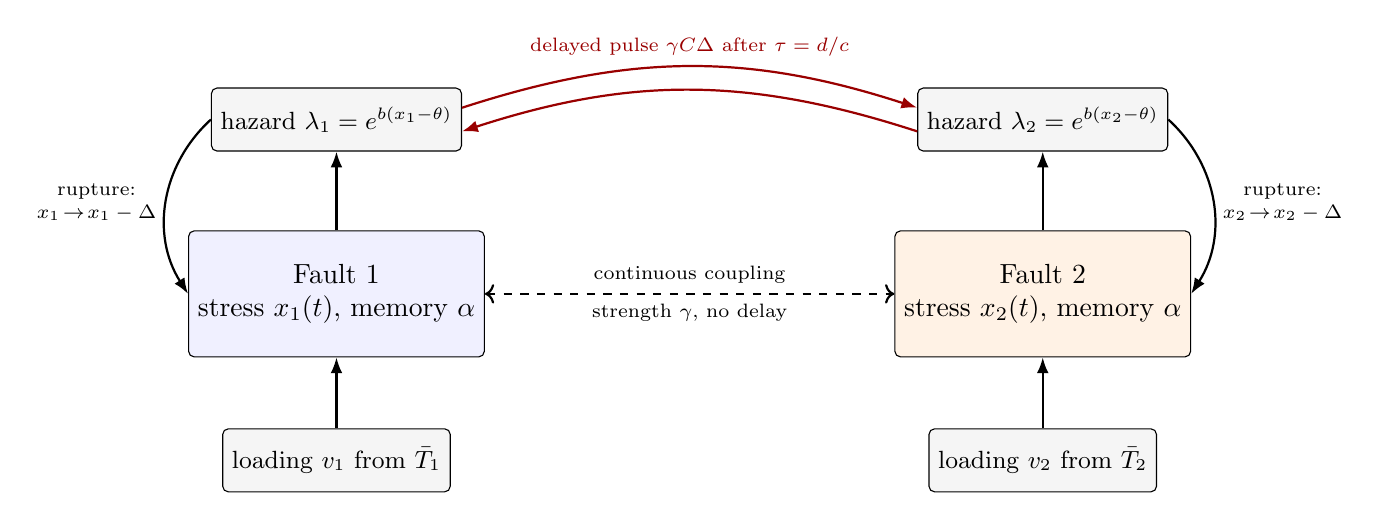
\begin{tikzpicture}[
  node distance=1.2cm,
  fault/.style={draw, rounded corners=2pt, minimum width=3.0cm, minimum height=1.6cm, align=center, fill=blue!6},
  fault2/.style={draw, rounded corners=2pt, minimum width=3.0cm, minimum height=1.6cm, align=center, fill=orange!10},
  proc/.style={draw, rounded corners=2pt, minimum width=2.6cm, minimum height=0.8cm, align=center, font=\small, fill=gray!8},
  arr/.style={-{Latex[length=2mm]}, thick},
  lab/.style={font=\scriptsize, align=center}
]
\node[fault] (F1) {Fault 1\\ stress $x_1(t)$, memory $\alpha$};
\node[fault2, right=5.2cm of F1] (F2) {Fault 2\\ stress $x_2(t)$, memory $\alpha$};
% continuous coupling
\draw[arr, <->, dashed] (F1.east) -- node[above, lab] {continuous coupling} node[below, lab] {strength $\gamma$, no delay} (F2.west);
% loading
\node[proc, below=0.9cm of F1] (L1) {loading $v_1$ from $\bar T_1$};
\node[proc, below=0.9cm of F2] (L2) {loading $v_2$ from $\bar T_2$};
\draw[arr] (L1) -- (F1);
\draw[arr] (L2) -- (F2);
% hazard and rupture
\node[proc, above=1.0cm of F1] (H1) {hazard $\lambda_1=e^{b(x_1-\theta)}$};
\node[proc, above=1.0cm of F2] (H2) {hazard $\lambda_2=e^{b(x_2-\theta)}$};
\draw[arr] (F1) -- (H1);
\draw[arr] (F2) -- (H2);
\draw[arr, bend right=40] (H1.west) to node[left, lab] {rupture:\\ $x_1\!\to\!x_1-\Delta$} (F1.west);
\draw[arr, bend left=40] (H2.east) to node[right, lab] {rupture:\\ $x_2\!\to\!x_2-\Delta$} (F2.east);
% delayed pulses
\draw[arr, red!60!black, bend left=18] ([yshift=0.15cm]H1.east) to node[above, lab, red!60!black] {delayed pulse $\gamma C\Delta$ after $\tau=d/c$} ([yshift=0.15cm]H2.west);
\draw[arr, red!60!black, bend right=18] ([yshift=-0.15cm]H2.west) to ([yshift=-0.15cm]H1.east);
\end{tikzpicture}
}
\caption{Model structure: fractional stress accumulation, exponential hazard, rupture reset and a delayed pulse to the neighbour; continuous coupling (dashed) is instantaneous.}\label{fig:schematic}
\end{figure}

\begin{figure}[t]
\centering\resizebox{\textwidth}{!}{\figCycle}
\caption{Left: stress cycles of one fault (illustrative shape). Without memory ($\alpha=1$, orange) stress saturates smoothly; with memory ($\alpha<1$, blue) it rises fast after a rupture and then creeps towards the threshold, giving a different recurrence pattern. A rupture removes $\Delta$. Right: the exponential hazard.}\label{fig:cycle}
\end{figure}

\begin{figure}[t]
\centering\resizebox{0.95\textwidth}{!}{\figDelay}
\caption{Delayed interaction. A rupture of fault 1 at $t_0$ changes fault 2 only at $t_0+\tau$, by $\gamma C\Delta$, which can advance the next rupture of fault 2.}\label{fig:delay}
\end{figure}


\begin{figure}[t]
\centering
\begin{minipage}{0.47\textwidth}\centering\includegraphics[width=\textwidth]{loading_calibration.pdf}\end{minipage}\hfill
\begin{minipage}{0.51\textwidth}\centering\includegraphics[width=\textwidth]{sim_dataset.pdf}\end{minipage}
\caption{Left: calibrated stress build-up of an isolated fault for three memory orders, all reaching $\theta$ at $\Tb=40$ years ($v$ changes with $\alpha$). Right: a simulated 400-year dataset (true $\alpha=0.7$, $\gamma=0.08$, $\tau=3$ yr, $b=3$); lines: latent stress, dots: yearly noisy observations, triangles: ruptures, dashed: threshold.}\label{fig:loading}
\end{figure}

\section{Inference}
The fractional kernel is completely monotone, so $t^{\alpha-1}/\Gamma(\alpha)\approx\sum_{k=1}^{K}w_ke^{-s_kt}$ ($K=21$ plus a tail term), which makes the system Markov and the cost linear in time. The likelihood of the yearly readings and rupture times is estimated by a bootstrap particle filter \citep{Gordon1993,DoucetJohansen2011} ($P=100$ particles, systematic resampling when ESS $<P/2$, common random numbers across parameter values). $(\alpha,\gamma,c,b)$ is estimated on the scale $(\mathrm{logit}\,\alpha,\log\gamma,\log c,\log b)$ by Nelder--Mead \citep{NelderMead1965} from several starts. Fixed: $\beta=0.05$, $\theta=10$, $\rho=0.2$, $\Tb=(40,45)$, $d=30$, $C=3$, $\sigma_x=0.1$, $\lambda_0=1$. The delay is identified only to the time step $h=0.25$ because pulses are applied at grid points.

\begin{figure}[t]
\centering\includegraphics[width=0.8\textwidth]{soe_kernel.pdf}
\caption{Fractional kernel and its sum-of-exponentials approximation for $\alpha=0.5,0.7,0.9$ (left) and pointwise relative error (right).}\label{fig:soe}
\end{figure}


\paragraph{Likelihood shape.}
Figure~\ref{fig:slices} shows one-dimensional slices of the estimated log-likelihood around the truth. $\alpha$, $\gamma$ and $b$ are sharply identified. The delay is identified \emph{only up to the time grid}: since pulses are applied at grid points, the likelihood is piecewise constant in $c$, and $\tau=d/c$ can be recovered to within the step $h$ at best. This is a property of the discretisation and is reported as such rather than hidden.

\begin{figure}[t]
\centering\includegraphics[width=0.95\textwidth]{slices.pdf}
\caption{Log-likelihood slices (relative to the truth) for $\alpha$, $\gamma$, delay $\tau=d/c$ and $b$, on one dataset; band = range over four common-random-number seeds. Dashed: true values. The delay panel is a step function because $\tau$ is resolved only to the grid step.}\label{fig:slices}
\end{figure}



\section{Statistical protocol}\label{sec:stats}
Data are simulated (400-year records, truth $(\alpha,\gamma,c,b)=(0.7,0.08,10,3)$, $\tau=3$ yr) in two scenarios: S1 with accurate readings ($\sigma_y=0.3$) and S2 with noisy readings ($\sigma_y=1.5$). \textbf{Recovery:} bias, SD and RMSE over replicates. \textbf{Memory:} $H_0:\alpha=1$ is on the boundary, so $\Lambda=2\{\ell(\hat\vartheta)-\ell(\hat\vartheta_{H_0})\}$ is compared with a parametric-bootstrap null ($B_0$ datasets under $\alpha=1$) rather than $\chi^2_1$ \citep{Chernoff1954,SelfLiang1987}. \textbf{Interaction:} $H_0:\gamma=0$ is also a boundary and $c$ is unidentified under $H_0$ \citep{Davies1977}; only the power against the $\chi^2_1$ reference is reported. \textbf{Robustness:} fits with $\Tb$ scaled by $0.8$ and $1.25$. \textbf{Forecasts:} on an independent record, the probability that each fault ruptures in the next $W=5$ years, scored by Brier, log score, AUC and Brier skill against Poisson, Weibull-renewal and no-memory ($\alpha=1$) benchmarks. A replicate is called \emph{valid} if its maximised log-likelihood is within two units of that at the true parameters (i.e.\ the optimiser did not stall); this uses the truth, so it is a diagnostic of the study, not a rule for real data.

\paragraph{Memory, $H_0:\alpha=1$.}
The null $\alpha=1$ is on the boundary of $(0,1]$. The likelihood-ratio statistic $\Lambda=2\{\ell(\hat\vartheta)-\ell(\hat\vartheta_{H_0})\}$ then does not have the $\chi^2_1$ limit; asymptotically one expects the mixture $\tfrac12\chi^2_0+\tfrac12\chi^2_1$ \citep{Chernoff1954,SelfLiang1987}, whose 95\% point is $2.71$. With a Monte Carlo likelihood, noise of order one log-likelihood unit and finite $T$, asymptotics are not trusted. We therefore calibrate the test by \emph{parametric bootstrap}: $B_0$ datasets are generated under $\alpha=1$ (with the other parameters at their truth), the full and restricted fits are computed on each, and the empirical 95\% quantile of $\Lambda$ is the critical value. We report the empirical size when using the $\chi^2$ reference, the bootstrap critical value, and the power at the true $\alpha=0.7$.

\paragraph{Profile likelihood.}
For the first replicates the profile log-likelihood of $\alpha$ is computed on a grid $\{0.40,0.45,\dots,1.0\}$ by maximising over $(\gamma,c,b)$ at each $\alpha$. The profile deviance $2\{\hat\ell-\ell_p(\alpha)\}$ is plotted; since the Monte Carlo noise of the particle filter (standard deviation of order $1$--$2$ log-likelihood units) is of the same order as the usual deviance thresholds, profile-based confidence intervals and their coverage are \emph{not} claimed.

\section{Results}\label{sec:results}
We use $R=24$ (S1) and $16$ (S2) replicates, $B_0=40/24$ null datasets and $12$ datasets for the robustness study.

\paragraph{Recovery.} Of the replicates, $19/24$ (S1) and $9/16$ (S2) are valid; the others are optimiser failures (below the log-likelihood of the truth), not information failures. Among valid ones (Table~\ref{tab:recovery}) $\alpha$, $\gamma$ and $c$ are essentially unbiased in S1 (relative RMSE $0.8\%$, $4.2\%$, $2.0\%$) while $b$ is biased downwards ($2.47$ for a true $3$). Under noise (S2) $\alpha$ is still recovered (relative RMSE $2.0\%$), but $c$, hence the delay, is the least well identified ($13\%$).

\begin{table}[t]
\centering\scriptsize
\input{\tabdir/tab_recovery.tex}
\caption{Recovery of $(\alpha,\gamma,c,b)$ over valid replicates ($19/24$ in S1, $9/16$ in S2).}\label{tab:recovery}
\end{table}

\paragraph{Tests.} The LR statistic for memory is very large under $\alpha=0.7$ (minimum $1380$ in S1, $344$ in S2), so the power of both tests is $100\%$ at this effect size (Table~\ref{tab:tests}). Under $H_0$, $\hat\alpha$ sits at the boundary (mean $0.992$, never below $0.98$). The $\chi^2_1$ cut-off $2.706$ is unreliable: its size is $30\%$ in S1 and $8\%$ in S2; the bootstrap $95\%$ points are $6.94$ and $2.98$. The coupling test is not calibrated; its power is reported only as a guide.

\begin{table}[t]
\centering\scriptsize
\input{\tabdir/tab_tests.tex}
\caption{Tests of memory and coupling. Type I: rejection rate of the $\chi^2_1$ cut-off under $H_0:\alpha=1$ ($B_0$ null datasets); crit.: bootstrap $95\%$ point; power over valid replicates.}\label{tab:tests}
\end{table}


\paragraph{Robustness.} A wrong $\Tb$ lowers the maximised log-likelihood by $134$ ($\times0.8$) and $91$ ($\times1.25$) units on average, so it is detectable, and it shifts $\hat\alpha$ ($0.69$, $0.77$), $\hat\gamma$ ($0.055$, $0.067$) and $\hat b$ ($2.3$, $2.2$): the \emph{presence} of memory is robust, its \emph{size} is not (Table~\ref{tab:misspec}).
\begin{table}[t]
\centering\scriptsize
\input{\tabdir/tab_misspec.tex}
\caption{Fits with a wrong reference recurrence time (12 S1 datasets; truth $0.7$, $0.08$, $10$, $3$). Loss: drop of the maximised log-likelihood.}\label{tab:misspec}
\end{table}

\paragraph{Forecasts.} In both scenarios the fitted fractional model has the lowest Brier score ($0.048$, $0.046$ against $0.072$ for Poisson and $0.064$ for Weibull) and the highest AUC ($0.94$), i.e.\ a Brier skill of $+33\%$ and $+35\%$ over Poisson (Table~\ref{tab:forecast}). The refit without memory is worse than Poisson ($-38\%$, $-168\%$), reflecting miscalibration of a misspecified model. \emph{Caveat:} the fractional model uses the stress readings while Poisson and Weibull use only the catalogue, so this shows the value of observing stress, not superiority at equal information.

\begin{table}[t]
\centering\scriptsize
\input{\tabdir/tab_forecast.tex}
\caption{Out-of-sample 5-year window forecasts ($24$ replicates in S1, $16$ in S2).}\label{tab:forecast}
\end{table}

\begin{figure}[t]
\centering\maybefig{forecast_eval.pdf}{0.9}{}
\caption{Reliability diagram (left), ROC curves (centre) and Brier skill against Poisson (right; mean $\pm$ SE).}\label{fig:forecast}
\end{figure}

\section{Answers to the research questions}\label{sec:answers}
\begin{description}\setlength\itemsep{2pt}
\item[RQ1 --- recovery.] \emph{Yes, with limits.} With accurate readings (S1) $\alpha$, $\gamma$ and $c$ are recovered with relative RMSE $0.8\%$, $4.2\%$ and $2.0\%$; $b$ is biased downwards ($2.47$ for a true $3$, relative RMSE $18\%$). With noisy readings (S2) $\alpha$ is still recovered ($2.0\%$), $\gamma$ and $b$ less well ($12\%$, $14\%$), and the delay speed $c$ worst ($13\%$). These figures are for valid fits only ($19/24$ and $9/16$ of the replicates), so they are optimistic.
\item[RQ2 --- memory.] \emph{Yes.} The LR statistic is far beyond any critical value (minimum $1380$ in S1, $344$ in S2), so the power is $100\%$ at $\alpha=0.7$. The $\chi^2_1$ calibration is \emph{not} valid: its size is $30\%$ (S1) and $8\%$ (S2); the parametric-bootstrap $95\%$ points are $6.94$ and $2.98$, and $\hat\alpha$ lies at the boundary under $H_0$ ($0.992$ on average).
\item[RQ3 --- interaction.] \emph{Suggestively yes.} The coupling statistic also gives power $100\%$, but $\gamma=0$ is a boundary and $c$ is unidentified under $H_0$, and this test is not bootstrap-calibrated, so the result shows only that a coupling of size $0.08$ is far from the null, not that the test has the nominal size.
\item[RQ4 --- robustness.] \emph{Partly.} A wrong $\Tb$ ($\times0.8$ or $\times1.25$) costs $134$ and $91$ log-likelihood units on average, so it is detectable; the \emph{presence} of memory survives, but $\hat\alpha$ ($0.69$, $0.77$), $\hat\gamma$ ($0.055$, $0.067$) and $\hat b$ ($2.3$, $2.2$) are shifted, so the \emph{size} of memory and coupling is not robust.
\item[RQ5 --- forecasts.] \emph{Yes against catalogue-based benchmarks, not yet at equal information.} The fitted model has Brier skill $+33\%$ (S1) and $+35\%$ (S2) over Poisson, against $+10.5\%$ for Weibull renewal, and AUC $0.94$ against $0.83$; with memory switched off it is worse than Poisson ($-38\%$, $-168\%$). Since the fractional model reads the stress while the benchmarks do not, this measures the value of observing stress together with the model structure.
\end{description}

\section{Discussion and limitations}
\begin{itemize}\setlength\itemsep{1pt}
\item \textbf{Stress is observed directly.} In the simulations the noisy stress itself is measured yearly. In reality only catalogues and proxies (geodetic strain etc.) are available, so the recovery results are an \emph{upper bound} on identifiability and S2 is the closer analogue. Real data require a proxy observation model.
\item \textbf{Optimiser failures.} $5/24$ (S1) and $7/16$ (S2) fits stalled below the likelihood of the truth; summaries keep valid fits only, with validity defined through the truth, which is optimistic and unusable on real data.
\item \textbf{Forecast comparison is not information-matched.} The fractional model uses stress readings; Poisson and Weibull do not. No ETAS or stress-release benchmark has been run.
\item \textbf{Boundary and nuisance-parameter problems.} Both $H_0:\alpha=1$ and $H_0:\gamma=0$ violate regularity conditions; only the first is bootstrap-calibrated, using other parameters at their true values.
\item \textbf{Monte Carlo noise and delay resolution.} The particle-filter log-likelihood has noise of $1$--$2$ units, comparable to deviance thresholds, so no coverage of profile intervals is claimed; $\tau$ is identified only to the grid step.
\item \textbf{Known structure.} Data come from the model class that is fitted; the $\Tb$ study probes misspecification only partly. Two faults, scalar stress and common $\alpha$ are simplifications of real fault networks.
\item \textbf{Forecasts are probabilities,} judged by calibration and skill, not by hitting individual events. The literature survey is not exhaustive and entries for other work come from abstracts or posted preprints; the Physica Scripta paper \citep{PhysScr2024} could not be accessed.
\end{itemize}
An improved protocol addressing the second, third and fourth points (multi-start optimiser with a convergence check that does not use the truth, an information-matched stress-regression benchmark, a bootstrap-calibrated coupling test, an automatically chosen neighbouring fault pair) is implemented in the accompanying code and will replace the numbers above.

\section{Conclusion}
We formulated a fractional, impulsive, delayed model of two interacting faults with a stress-dependent hazard, a calibrated loading rate and a particle-filter likelihood, and evaluated estimation accuracy, a boundary-aware memory test, robustness and out-of-sample probabilistic forecasts in simulation. The next steps are an observation model based on real proxies, finer or event-driven delay handling, and application to a real catalogue.

\paragraph{Reproducibility.} Python/numba code, scripts and notebooks: \url{https://github.com/yamenetoo/fractional-delayed-fault-model}. Seeds: $1000+r$ (alternative), $3000+r$ (null), $5000+r$ (forecast evaluation).

\begin{thebibliography}{99}\small
\bibitem[Burridge and Knopoff(1967)]{BurridgeKnopoff1967} Burridge, R., Knopoff, L. (1967). Model and theoretical seismicity. \emph{Bull. Seismol. Soc. Am.} 57(3), 341--371.
\bibitem[Bebbington and Harte(2003)]{Bebbington2003} Bebbington, M., Harte, D.S. (2003). The linked stress release model for spatio-temporal seismicity: formulations, procedures and applications. \emph{Geophys. J. Int.} 154, 925--946.
\bibitem[Chishtie(2026)]{Chishtie2026} Chishtie, F.A. (2026). A hierarchical fractional $N$-body framework for Coulomb stress evolution in fault networks: exact analytical solutions and falsifiable seismicity scaling laws. \emph{EGUsphere} 2026, 1--29 (preprint, not peer reviewed), doi:10.5194/egusphere-2026-3498.
\bibitem[Dahm and Hainzl(2022)]{DahmHainzl2022} Dahm, T., Hainzl, S. (2022). A Coulomb stress response model for time-dependent earthquake forecasts. \emph{J. Geophys. Res. Solid Earth} 127(9), doi:10.1029/2022JB024443.
\bibitem[Demir and Kocy{\i}{\u g}it(2025)]{DemirKocyigit2025} Demir, T., Kocy{\i}{\u g}it, A. (2025). Seismic wave propagation in viscoelastic media under Atangana--Baleanu fractional dynamics: model formulation and numerical simulations. arXiv:2512.13897.
\bibitem[Dieterich(1994)]{Dieterich1994} Dieterich, J. (1994). A constitutive law for rate of earthquake production and its application to earthquake clustering. \emph{J. Geophys. Res.} 99(B2), 2601--2618.
\bibitem[Lu and Vere-Jones(2000)]{LuVereJones2000} Lu, C., Vere-Jones, D. (2000). Application of linked stress release model to historical earthquake data: comparison between two kinds of tectonic seismicity. \emph{Pure Appl. Geophys.} 157, 2351--2364.
\bibitem[Matthews et al.(2002)]{Matthews2002} Matthews, M.V., Ellsworth, W.L., Reasenberg, P.A. (2002). A Brownian model for recurrent earthquakes. \emph{Bull. Seismol. Soc. Am.} 92, 2233--2250.
\bibitem[Anonymous(2024)]{PhysScr2024} \emph{Delayed and fractional-order dynamics of a model for earthquake induced by stress perturbations}. \emph{Physica Scripta} (2024), doi:10.1088/1402-4896/ad20ba. [authors and details to be added; full text not accessed]
\bibitem[Stein(1999)]{Stein1999} Stein, R.S. (1999). The role of stress transfer in earthquake occurrence. \emph{Nature} 402, 605--609.
\bibitem[Styron and Pagani(2020)]{StyronPagani2020} Styron, R., Pagani, M. (2020). The GEM Global Active Faults Database. \emph{Earthquake Spectra} 36(1\_suppl), 160--180.
\bibitem[Vere-Jones(1978)]{VereJones1978} Vere-Jones, D. (1978). Earthquake prediction---a statistician's view. \emph{J. Phys. Earth} 26, 129--146.
\bibitem[Zheng and Vere-Jones(1991)]{ZhengVereJones1991} Zheng, X., Vere-Jones, D. (1991). Application of stress release models to historical earthquakes from North China. \emph{Pure Appl. Geophys.} 135, 559--576.
\bibitem[Chernoff(1954)]{Chernoff1954} Chernoff, H. (1954). On the distribution of the likelihood ratio. \emph{Ann. Math. Statist.} 25, 573--578.
\bibitem[Davies(1977)]{Davies1977} Davies, R.B. (1977). Hypothesis testing when a nuisance parameter is present only under the alternative. \emph{Biometrika} 64, 247--254.
\bibitem[Diethelm(2010)]{Diethelm2010} Diethelm, K. (2010). \emph{The Analysis of Fractional Differential Equations}. Springer.
\bibitem[Doucet and Johansen(2011)]{DoucetJohansen2011} Doucet, A., Johansen, A.M. (2011). A tutorial on particle filtering and smoothing: fifteen years later. In \emph{Oxford Handbook of Nonlinear Filtering}.
\bibitem[Gordon et al.(1993)]{Gordon1993} Gordon, N.J., Salmond, D.J., Smith, A.F.M. (1993). Novel approach to nonlinear/non-Gaussian Bayesian state estimation. \emph{IEE Proc. F} 140(2), 107--113.
\bibitem[Hawkes(1971)]{Hawkes1971} Hawkes, A.G. (1971). Spectra of some self-exciting and mutually exciting point processes. \emph{Biometrika} 58, 83--90.
\bibitem[Nelder and Mead(1965)]{NelderMead1965} Nelder, J.A., Mead, R. (1965). A simplex method for function minimization. \emph{Comput. J.} 7, 308--313.
\bibitem[Ogata(1988)]{Ogata1988} Ogata, Y. (1988). Statistical models for earthquake occurrences and residual analysis for point processes. \emph{J. Amer. Statist. Assoc.} 83, 9--27.
\bibitem[Podlubny(1999)]{Podlubny1999} Podlubny, I. (1999). \emph{Fractional Differential Equations}. Academic Press.
\bibitem[Self and Liang(1987)]{SelfLiang1987} Self, S.G., Liang, K.-Y. (1987). Asymptotic properties of maximum likelihood estimators and likelihood ratio tests under nonstandard conditions. \emph{J. Amer. Statist. Assoc.} 82, 605--610.
\end{thebibliography}
\end{document}
